\section{Background}
\label{sec:background}
Distributed systems and centralized systems alike, need to preserve the temporal order of events produced by concurrent processes in the system. When there are separated processes that can only communicate through messages, you cannot easily order these messages.
Therefore we need ordering algorithms to overcome this problem.
\par
We have two types of ordering algorithms \autocite{lamport1978time}: the partial order algorithms and the total order algorithms.
\subsection{Partial Order Algorithms}
Assuming S is partially ordered under $\leq$, then the following statements hold for all a, b and c in S:
\begin{itemize}
	\item Reflexivity: $a \leq a$ for all $a \in S$.
	\item Antisymmetry: $a \leq b$ and $b \leq a$ implies $a=b$ .
	\item Transitivity: $a \leq b$  and $b \leq c$  implies $a \leq c$.
\end{itemize}

\subsection{Total Order Algorithms}
A totally ordered set of events is a partially ordered set which satisfies one additional property:
\begin{itemize}
	\item Totality (trichotomy law): For any $a, b \in S$, either $a \leq b$  or $b \leq a$.
\end{itemize}
\par
In other words, total order is an ordering that defines the exact order of every event in the system. On the other hand, partial ordering only defines the order between certain key events that depend on each other. Partial order can be useful since it is less costly to implement. However, in some cases the order of all events is important. For example, imagine we have multiple databases around the world. We want them to appear as if it is only one database. To achieve this, every operation done a particular database would have to be replicated on all the others, we would then have to make sure that every operation is executed in the same order on every database to end up in the same state. However, Total Order is not usually scalable. This lead to the emergence of most of the work on eventual consistency. \epto claims to solve this issue.

\subsection{\epto Architecture}
\begin{figure}[htp]
	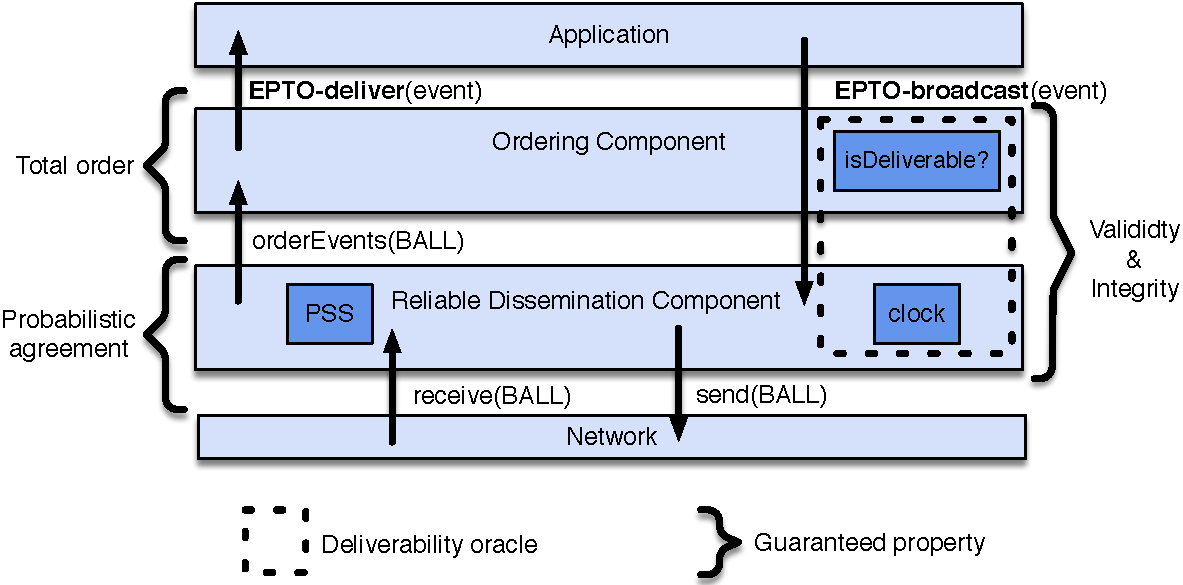
\includegraphics[width=\linewidth]{figures/architecture.pdf}
	\caption{\epto architecture \autocite{matos2015epto}.}
	\label{fig:epto-architecture}
\end{figure}
\autoref{fig:epto-architecture} illustrates the architecture of a single \epto replica. An application extending our Application class can \epto-broadcast and \epto-deliver events. Events broadcasted to the Dissemination component are sent over the network every $\delta$ period, where $\delta$ is a unit of time. Every ball received from the network is unwrapped and its events are analyzed by the dissemination component to find out whether they need to be propagated further or not according to their Time To Live (TTL). They are then sent to the ordering component so that \epto can determine whether to deliver these events or not and in which order. The order is based on the \textit{timestamp} of the events given by the logical clock and their \textit{broadcasterID} in case of a tie. The network layer is managed by \eptotester.
\subsection{Related Work}
Related work concerning Total Order is already extensively covered in \autocite{matos2015epto}. \jt{Is this sufficient or should I recap everything presented in \autocite{matos2015epto}?}

Both \autocite{Chandra2007} and \autocite{Maia2011} extensively test a particular large scale distributed system. However, they do not offer a framework to benchmark different systems. \autocite{Leonini2009} presents a framework named SPlay to deploy such applications. Unfortunately, SPlay only allows for LUA applications to run. \eptotester offers a convenient architecture to deploy distributed applications regardless of the programming language used, provided they run in a docker container.
